\subsection{Key-Value Store Accelerator}

\begin{center}
\includegraphics[width=0.9\linewidth]{../../img/kvstore.pdf}
\end{center}

\subsubsection{Lookup Pipeline}

The main part of the accelerator is a lookup pipeline, which takes keys in
through an input interface and streams out the values through an output
interface. Each interface consists of two decoupled interfaces with ready-valid
signals. The first decoupled interface sends the length of the data to come,
and the second sends the data itself eight bits at a time.

When a key comes into the accelerator, the first thing done is to compute a
primary and secondary hash value. The hash algorithm used is the Pearson
hashing algorithm, a non-cryptographic hashing algorithm implemented as follows.

\begin{verbatim}
    h = array of size n
    for j from 0 to n-1
        h[j] = T[(x[0] + j) & 0xff]
        for i from 1 to length(x) - 1
            h[j] = T[h[j] ^ x[i]]
\end{verbatim}

In this algorithm, \(h\) is one byte in the final hash value,
\(x\) is the message, and \(T\) is a table containing a random permutation of
all the integers from 0 to 255. We use two different tables in order to
generate two different hash values, a primary and a secondary hash. When the
hasher is finished, it passes these two hashes to the key comparison unit.

The key comparison unit uses the hash value to index into the key memory.
The key memory reserves 256 bytes for each key, so the starting address of a
key in the memory can be found simply by taking the hash value and shifting it
to the right by a certain number of bits (the shift amount depends on the
word size of the memory, which can be parameterized).

If one of the two possible keys matches, the correct hash value is then passed
to the value memory unit. The value memory will then look up the value and
stream it out through the output interface. If neither of the two keys matched,
the value memory unit will send a zero through the length interface to
indicate that no value was found.

\subsubsection{Control through RoCC interface}

The accelerator is configured from software through the RoCC command interface.
To place a key into the accelerator, the lookup pipeline must first be
placed into write mode. In this mode, the hasher will no longer take keys
from the traffic manager, but will instead take the key from the memory handler,
which reads in the keys from DRAM through the RoCC memory interface.

Once the key is read in and hash values computed, the key compare unit will
then determine which hash slot the key can be placed in. A key can be placed
in a hash slot if the slot is empty, the key in the slot is the same as the
key to be placed, or the key has a lower weight than the key being placed.
The weight is simply a saturating count of how frequently the key is accessed.
The count can be reset from software so that keys which were once popular but
are no longer can be evicted.

Once the lookup pipeline has determined where the new key can be placed, the
controller will instruct the memory handler to read the value through the
RoCC memory interface and write it into the value memory.
